%% LaTeX-Beamer template for KIT design
%% by Erik Burger, Christian Hammer
%% title picture by Klaus Krogmann
%%
%% version 2.0
%%
%% mostly compatible to KIT corporate design v2.0
%% http://intranet.kit.edu/gestaltungsrichtlinien.php
%%
%% Problems, bugs and comments to
%% burger@kit.edu

\documentclass[18pt]{beamer}
\usetheme{kit}

%% TITLE PICTURE

% if a custom picture is to be used on the title page, copy it into the 'logos'
% directory, in the line below, replace 'mypicture' with the 
% filename (without extension) and uncomment the following line
% (picture proportions: 63 : 20, *.eps format if you use latex+dvips+ps2pdf,
% *.jpg/*.png/*.pdf if you use pdflatex)

%\titleimage{mypicture}

%% TITLE LOGO

% for a custom logo on the front page, copy your file into the 'logos'
% directory, insert the filename in the line below and uncomment it

%\titlelogo{mylogo}

% (*.eps format if you use latex+dvips+ps2pdf,
% *.jpg/*.png/*.pdf if you use pdflatex)

%% BIBTEX ICON/KEY

% if you want to see BibTeX keys in the references view instead of the symbol,
% uncomment the following line
% \usebibitemtemplate{\insertbiblabel}

% the presentation starts here

\title[Short title]{Tutorium 01: Projektplanung }
\subtitle{Softwaretechnik im SS 2011, Tutorien 4 + X + Y}
\author{Jürgen Walter}

\institute{Chair for Software Design and Quality}

\begin{document}

% change the following line to "ngerman" for German style date and logos
% change the following line to "english" for English style date and logos
\selectlanguage{ngerman}

%title page
\begin{frame}
\titlepage
\end{frame}

\section{Organisatorisches}

\subsection{Vorstellung}
\frame{
\frametitle{Wer bin ich?}
\begin{itemize}
\item Jürgen Walter
\pause
\item 8tes Semester Informatik
\pause
\item juergen.walter.halle@gmail.com
\item uxccx@student.kit.edu
\pause
\item Partnerturoren Christian Juelg und Daniel Deckers
\item \dots
\end{itemize}
}

%table of contents
\frame{
\frametitle{Was machen wir heute?}
\tableofcontents
}

\subsection{Übungsschein}
\frame{
\frametitle{Übungsschein}
\begin{block}{Der Übungsschein \dots}
\begin{itemize}
\pause
\item ist keine Vorraussetzung zur Klausur, aber Vorraussetzung für Modul!
\pause
\item hat 6 Übungsblätter mit  insgesammt 150 Punkten
\pause
\item ist mit 50 Prozent aus Übungsblättern und Programmmieraufgaben bestanden 
\end{itemize}
\end{block}
}


\section{Altes Übungsblatt und Wiederholungen}

\subsection{Zum Aufwärmen ...}
\frame {
\frametitle{Zeigt mal was ihr könnt, wahr oder falsch?}
\begin{itemize}
	\color<2-5>[rgb]{0,1,0}
	\item In der Planungsphase wird die softwaretechnische Realisierbarkeit eines Produktes untersucht
	\color[rgb]{0,0,0}
	\pause
	\color<3-5>[rgb]{1,0,0}
	\item Ein Pflichtenheft beschreibt die Eigenschaften, die das Produkt aus der Sicht des Kunden erfüllen soll
	\color[rgb]{0,0,0}
	\pause
	\color<4-5>[rgb]{0,1,0}
	\item In einem UML-Anwendungsfalldiagramm werden typische Interaktionen des Benutzers mit dem System modelliert
	\color[rgb]{0,0,0}
\end{itemize}
}


\subsection{Werkzeuge}

\frame{
\frametitle{Versionsverwaltungen}

\begin{block}{Subversion}
\begin{itemize}
\item von der Vorlesung unterstützte Versionsverwaltung
\item Windows: Tortoise SVN
\item Linux: Shell oder Tortoise SVN
\item Mac: Shell
\end{itemize}
\end{block}
\pause

\begin{block}{Git}
\begin{itemize}
\item Werkzeug des Tutors ;-)
\end{itemize}
\end{block}
}

\frame{
\frametitle{Checkstyle}
\begin{alertblock}{Das geht besser \dots}
\begin{itemize}
\item Keiner von euch ist ohne Checkstyle Fehler
\end{itemize}
\end{alertblock}
}



\subsection{Lastenheft}

\frame{
\frametitle{Lastenheft}
\begin{itemize}
\item enthält die Hauptanforderungen an das Produkt (user requirements)
\item formuliert mit natürlicher Sprache, evtl. Diagramme
\item dient der Kommunikation mit dem Kunden und der Projektplanung
\end{itemize}
}

\frame{
\frametitle{Lastenheft}
\begin{block}{Gliederungsschema Lastenheft}
\begin{itemize}
\item1.Zielbestimmung
\item2.Produkteinsatz
\item3.Funktionale Anforderungen
\item4.Produktdaten
\item5.Nichtfunktionale Anforderungen
\item6.Qualitätsanforderungen
\item   a)Szenarien
\item   b)Anwendungsfälle
\item7.Systemmodelle
\item8.Glossar (Begriffslexikon zur Beschreibung des Produktes)
\end{itemize}
\end{block}
}



\section{Ende}

\frame{
\frametitle{Tipps zum nächsten Übungsblatt}

\begin{block}{Aufgabe 1}
\begin{itemize}
\item Bla bla
\item Bla bla
\end{itemize}
\end{block}

\begin{block}{Aufgabe 2}
\begin{itemize}
\item Bla bla
\item Bla bla
\end{itemize}
\end{block}

\begin{block}{Aufgabe 3}
\begin{itemize}
\item Bla bla
\item Bla bla
\end{itemize}
\end{block}


}


\frame{
\frametitle{Bis zum nächsten Mal}
\begin{center}
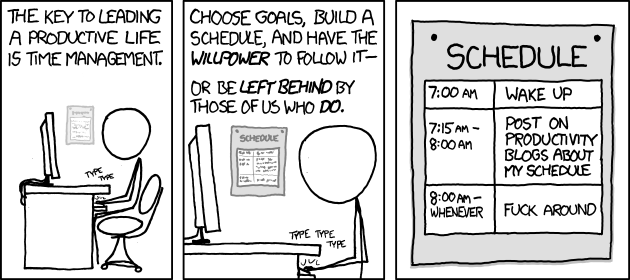
\includegraphics[width=1\textwidth]{pics/time_management}
\end{center}

}


\end{document}
